% !TEX TS-program = xelatex

% Copyright 2010 by Pedro Furlanetto 
%
% In principle, this file can be redistributed and/or modified under
% the terms of the GNU Public License, version 2.

% Based on Till Tantau beamer template

\documentclass{beamer}
%\documentclass[draft]{beamer}

\mode<presentation>
{
  \usetheme{Warsaw}
  \setbeamercovered{transparent}
}


\usepackage{graphicx}
\usepackage[english]{babel}
%\usepackage[utf8]{inputenc}
\usepackage{times}
\usepackage[T1]{fontenc}
\usepackage{xltxtra} % Extra customizations for XeLaTeX
\usepackage{color}
\usepackage{listings}
 

% "define" Scala
\lstdefinelanguage{Scala}{
  morekeywords={abstract,case,catch,class,def,%
    do,else,extends,false,final,finally,%
    for,if,implicit,import,match,mixin,%
    new,null,object,override,package,%
    private,protected,requires,return,sealed,%
    super,this,throw,trait,true,try,%
    type,val,var,while,with,yield},
  otherkeywords={=>,<-,<\%,<:,>:,\#,@},
  sensitive=true,
  morecomment=[l]{//},
  morecomment=[n]{/*}{*/},
  morestring=[b]",
  morestring=[b]',
  morestring=[b]"""
}


\definecolor{dkgreen}{rgb}{0,0.6,0}
\definecolor{gray}{rgb}{0.5,0.5,0.5}
\definecolor{mauve}{rgb}{0.58,0,0.82}

% Default settings for code listings
\lstset{frame=tb,
  language=Scala,
  aboveskip=3mm,
  belowskip=3mm,
  showstringspaces=false,
  columns=flexible,
  basicstyle={\small\ttfamily},
  numbers=none,
  numberstyle=\tiny\color{gray},
  keywordstyle=\color{blue},
  commentstyle=\color{dkgreen},
  stringstyle=\color{mauve},
  frame=single,
  breaklines=true,
  breakatwhitespace=true
  tabsize=3
}

\setbeamertemplate{navigation symbols}{}%remove navigation symbols

\title{Scala relâmpago}

\subtitle{Preciso de um subtítulo descritivo}

\author{Pedro Furlanetto}

\institute
{
  Ideais Tecnologia\\
  
\includegraphics[height=2cm]{ideais-grande.jpg} 
}

\date[IC 2010] % (optional, should be abbreviation of conference name)
{IdeaisConf, 2010}

\subject{Linguagem de Programação Scala}

%\logo{
\includegraphics[height=1cm]{ideais-grande.jpg}}

\AtBeginSubsection[]
{
  \begin{frame}<beamer>{Resumo}
    \tableofcontents[currentsection,currentsubsection,sectionstyle=show/shaded,subsectionstyle=show/shaded/shaded]
  \end{frame}
}

%\beamerdefaultoverlayspecification{<+->}

\begin{document}

\begin{frame}  
  \centering{
\includegraphics[height=1cm]{Scala_Logo2008.png}}\\
  \titlepage
\end{frame}

%\begin{frame}{Resumo}
%  \tableofcontents
%\end{frame}

\section{Overview}

\subsection{De onde veio}

\begin{frame}{Criada por}
	\begin{itemize}
	\item Martin Odersky - \emph{École Polytechnique Fédérale de Lausanne} (EPFL), Lausanne, Switzerland em 2001
	\begin{itemize}
	   \item Ph.D. com \emph{Niklaus Wirth} (criador do Pascal)
              \item \emph{GJ} e \emph{Pizza} com \emph{Philip Wadler} - deu origem ao \emph{generics} do Java atual
	\end{itemize}	
	\end{itemize}
           \begin{columns}
           \begin{column}{.5\textwidth}
               \centering{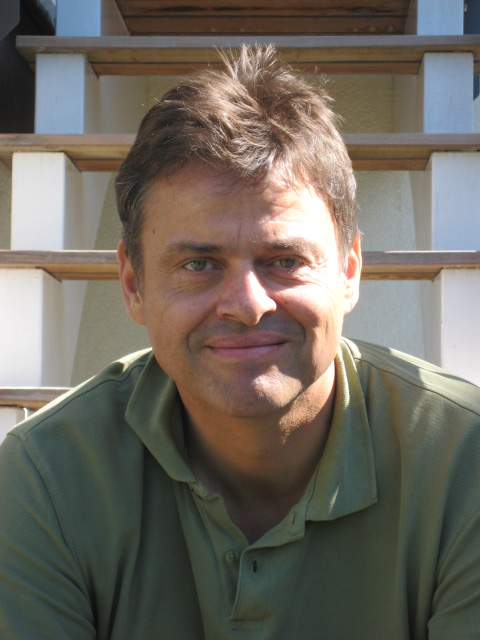
\includegraphics[height=4cm]{Martin-Odersky.jpg}}
           \end{column}
           \begin{column}{.5\textwidth}
               \centering{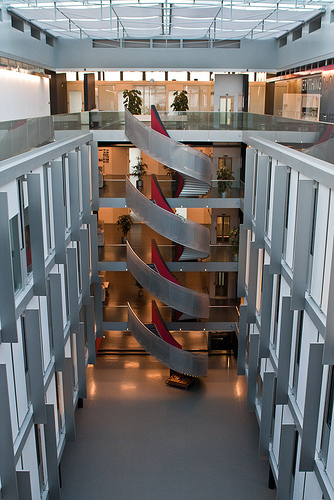
\includegraphics[height=4cm]{scala-the-real-thing.jpg}}
           \end{column}
	\end{columns}
\end{frame}

\subsection{O que é Scala?}

\begin{frame}{Unifica funcional e orientação a objeto} 
    \centering{ 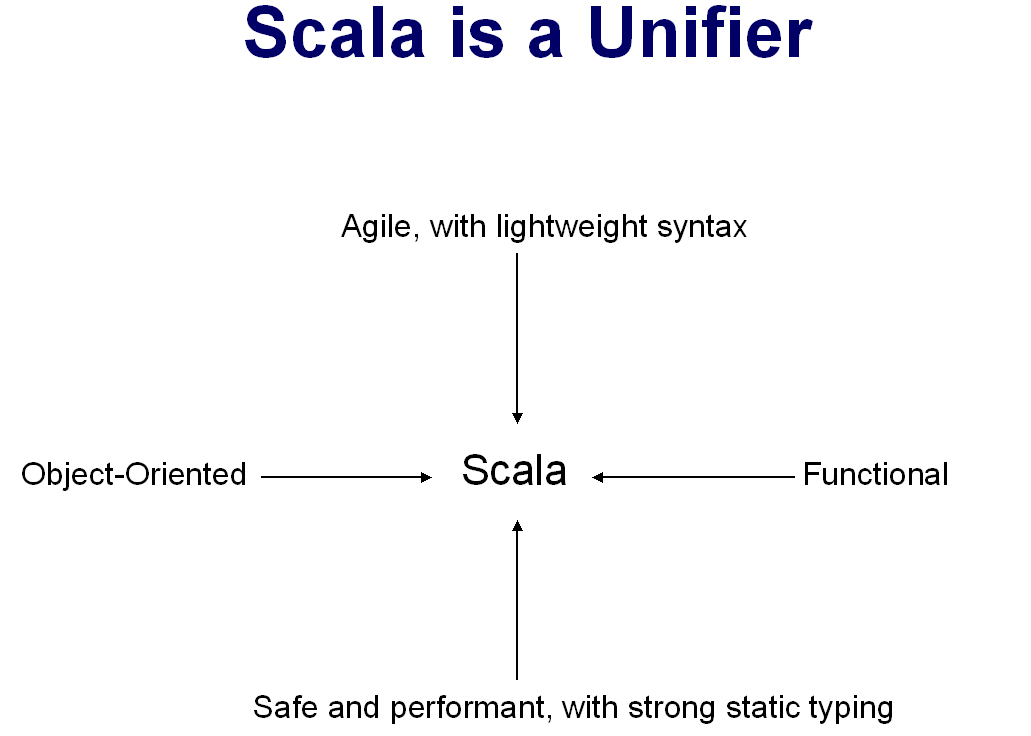
\includegraphics[scale=0.20]{Scala-is-a-Unifier.png}   } 
\end{frame}

\begin{frame}[fragile]{Algumas características} 
    \begin{itemize} %[<+->]
        \item Sintaxe simples e consistente 
        \begin{itemize}
              \item Exemplo: imports em qualquer lugar limitados pelo escopo 
        \end{itemize}
        \item Baseado em expressões
        \item Tudo são objetos e chamada de métodos (ala \emph{Smalltalk})
             \begin{lstlisting}
                 1 + 5 * 4 == 1.(5.*(4))
             \end{lstlisting}
        \item Métodos podem ser ``operadores''
        \item Closures e funções como \emph{first-class citizens}
             \begin{lstlisting}
                 val int2String =  (i:Int) => i.toString
             \end{lstlisting}
         \item Herança múltipla com \emph{traits e mixins}
    \end{itemize}
\end{frame}

\subsection{Será que é complicado?}

\begin{frame}{Será que é complicado?}
	\begin{columns}
           \begin{column}{.5\textwidth}               
              \centering{``\emph{Com grandes poderes vêm grandes responsabilidades.}''}
           \end{column}
           \begin{column}{.5\textwidth}
               
\includegraphics[height=5cm]{spiderman.png}
           \end{column}
	\end{columns}

\end{frame}
 
\begin{frame}[fragile] {Sample Scala}

    \begin{lstlisting}
    val t = "hello" 
    val x = 42 
    \end{lstlisting}

\end{frame}

\begin{frame}{Columns and Alignment}
     \begin{columns}[t] % contents are top vertically aligned
     \begin{column}[T]{5cm} % each column can also be its own environment
     Contents of first column \\ split into two lines
     \end{column}
     \begin{column}[T]{5cm} % alternative top-align that's better for graphics
         % \includegraphics[height=3cm]{graphic.png}
	Contents of second column with bigger line to see how break works
     \end{column}
     \end{columns}
\end{frame}



\begin{frame}{Blocks}
 
   \begin{block}{This is a Block}
      This is important information
   \end{block}
 
   \begin{alertblock}{This is an Alert block}
   This is an important alert
   \end{alertblock}
 
   \begin{exampleblock}{This is an Example block}
   This is an example 
   \end{exampleblock}
 
\end{frame}





\begin{frame}{Make Titles Informative. Use Uppercase Letters.}{Subtitles are optional.}
  % - A title should summarize the slide in an understandable fashion
  %   for anyone how does not follow everything on the slide itself.

  \begin{itemize}
  \item
    Use \texttt{itemize} a lot.
  \item
    Use very short sentences or short phrases.
  \end{itemize}
\end{frame}

\begin{frame}{Make Titles Informative.}

  You can create overlays\dots
  \begin{itemize}
  \item using the \texttt{pause} command:
    \begin{itemize}
    \item
      First item.
      \pause
    \item    
      Second item.
    \end{itemize}
  \item
    using overlay specifications:
    \begin{itemize}
    \item<3->
      First item.
    \item<4->
      Second item.
    \end{itemize}
  \item
    using the general \texttt{uncover} command:
    \begin{itemize}
      \uncover<5->{\item
        First item.}
      \uncover<6->{\item
        Second item.}
    \end{itemize}
  \end{itemize}
\end{frame}



\section{Our Results/Contribution}

\subsection{Main Results}

\begin{frame}{Make Titles Informative.}
\end{frame}

\begin{frame}{Make Titles Informative.}
\end{frame}

\begin{frame}{Make Titles Informative.}
\end{frame}


\subsection{Basic Ideas for Proofs/Implementation}

\begin{frame}{Make Titles Informative.}
\end{frame}

\begin{frame}{Make Titles Informative.}
\end{frame}

\begin{frame}{Make Titles Informative.}
\end{frame}



\section*{Summary}

\begin{frame}{Summary}

  % Keep the summary *very short*.
  \begin{itemize}
  \item
    The \alert{first main message} of your talk in one or two lines.
  \item
    The \alert{second main message} of your talk in one or two lines.
  \item
    Perhaps a \alert{third message}, but not more than that.
  \end{itemize}
  
  % The following outlook is optional.
  \vskip0pt plus.5fill
  \begin{itemize}
  \item
    Outlook
    \begin{itemize}
    \item
      Something you haven't solved.
    \item
      Something else you haven't solved.
    \end{itemize}
  \end{itemize}
\end{frame}



% All of the following is optional and typically not needed. 
\appendix
\section<presentation>*{\appendixname}
\subsection<presentation>*{For Further Reading}

\begin{frame}[allowframebreaks]
  \frametitle<presentation>{For Further Reading}
    
  \begin{thebibliography}{10}
    
  \beamertemplatebookbibitems
  % Start with overview books.

  \bibitem{Author1990}
    A.~Author.
    \newblock {\em Handbook of Everything}.
    \newblock Some Press, 1990.
 
    
  \beamertemplatearticlebibitems
  % Followed by interesting articles. Keep the list short. 

  \bibitem{Someone2000}
    S.~Someone.
    \newblock On this and that.
    \newblock {\em Journal of This and That}, 2(1):50--100,
    2000.
  \end{thebibliography}
\end{frame}

\end{document}


